\documentclass[9pt,a4paper]{extarticle}
\usepackage{amsmath,amssymb,amsfonts}
\usepackage[margin=0.6in]{geometry}
\usepackage{booktabs}
\usepackage{graphicx}
\usepackage[font=small,labelfont=bf]{caption}
\usepackage{microtype}
\pagestyle{empty}
\setlength{\parskip}{2pt}
\setlength{\parindent}{0pt}
\abovedisplayskip=4pt \belowdisplayskip=4pt
\abovedisplayshortskip=2pt \belowdisplayshortskip=2pt

\def\R{\mathbb{R}}
\def\E{\mathbb{E}}
\def\N{\mathcal{N}}

\begin{document}

{\large\bfseries Bridge sampling schemes, and what separates them}\hfill
{\small normalised time $s=t/T\in[0,1]$}
\vspace{2pt}\hrule\vspace{4pt}

\textbf{The process.} Source $x\sim\Phi=\N(0,I)$, target $y\sim\Psi$, driver
$Z_t=x+\sigma W_t$. The $\Phi$-initialised Gaussian random bridge to $\Psi$ is
$\xi_t\mid(x,y)\sim\N\big(x+\tfrac{t}{T}(y-x),\,\sigma^2\tfrac{t(T-t)}{T}I\big)$, i.e.
\begin{equation}
\xi_s=(1-s)x+sy+\gamma\sqrt{s(1-s)}\,\varepsilon,\qquad
\varepsilon\sim\N(0,I),\quad \gamma^2:=\sigma^2T .
\end{equation}
\emph{$\sigma$ and $T$ are not separately identifiable} --- training and sampling
depend on them only through $\gamma$; the published $\sigma=1,T=0.1$ is
$\gamma=0.3162$. The network regresses the endpoint,
$f_\theta(\xi_s,s)\approx\E[Y\mid\xi_s]$, under $\E\|y-f_\theta\|^2$ with
$s\sim\mathcal{U}[0,1)$ --- not a score, not a noise prediction. The
non-anticipative dynamics are
\begin{equation}
\label{eq:sde}
\mathrm{d}\xi_s=\frac{\E[Y\mid\xi_s]-\xi_s}{1-s}\,\mathrm{d}s+\gamma\,\mathrm{d}B_s .
\end{equation}

\vspace{1pt}\hrule\vspace{4pt}

\textbf{Three samplers.} With $\hat y=f_\theta(\xi_s,s)$, advancing $s\to u$; each
costs one network evaluation.

\emph{(a) Euler--Maruyama} --- Algorithm 2 of the manuscript, a discretisation of
\eqref{eq:sde}: $\ \xi_u=\xi_s+\tfrac{\hat y-\xi_s}{1-s}(u-s)+\gamma\sqrt{u-s}\,z$,
$z\sim\N(0,I)$.

\emph{(b) Deterministic Euler} --- \eqref{eq:sde} with the diffusion deleted;
\textbf{this is what the original code evaluated} (\texttt{sample\_bridges.py}
passes \texttt{deterministic=True}): $\ \xi_u=\xi_s+\tfrac{\hat y-\xi_s}{1-s}(u-s)$.
It is \emph{biased}. A deterministic sampler preserving the marginals of
\eqref{eq:sde} must follow the probability-flow ODE, with drift
$b(\xi,s)-\tfrac{\gamma^2}{2}\nabla\!\log p_s(\xi)$; dropping $\gamma\,\mathrm{d}B_s$
without that score correction gives neither the SDE nor its flow ODE, so refining
the grid converges to the wrong law. The symptom is under-dispersion, and it is
the reported step-count plateau.

\emph{(c) Exact bridge posterior} --- recommended. Given $\xi_s$ and $\hat y$, the
law of $\xi_u$ under the Brownian bridge pinned at $(s,\xi_s)$ and $(1,\hat y)$ is
exactly
\begin{equation}
\xi_u\sim\N\!\left(\xi_s+\tfrac{u-s}{1-s}(\hat y-\xi_s),\
\gamma^2\tfrac{(u-s)(1-u)}{1-s}I\right).
\end{equation}
The variance vanishes at $u=1$: the terminal point is hit exactly, with no
$1/(T-t)$ singularity, no boundary offset, and no time-discretisation error. To
first order in $(u-s)$ it agrees with (a), so it is the exact form of the same
dynamics.

\emph{Flow matching} is the $\gamma\to0$, velocity-parameterised member of this
family: the interpolant becomes $(1-s)x+sy$ and the targets are related by
$v=(\hat y-\xi_s)/(1-s)$. A matched-budget comparison therefore isolates exactly
the stochastic latent and the parameterisation.

\vspace{1pt}\hrule\vspace{4pt}

\textbf{One sampler, three drivers.} Scheme (c) needs only the bridge transition
kernel, never the martingale $\{M_t\}$ on which the manuscript's L\'evy section is
gated. Substituting other L\'evy marginals gives closed forms with the \emph{same}
drift $\xi_s+(\hat y-\xi_s)\tfrac{u-s}{1-s}$ and only the fluctuation changing:

\vspace{-3pt}
\begin{center}\small
\begin{tabular}{llll}
\toprule
Driver & Exact transition $\xi_s\to\xi_u$ & Support & Parameter\\
\midrule
Brownian & $\N\big(\text{drift},\,\gamma^2\frac{(u-s)(1-u)}{1-s}\big)$ & $\R$ & $\gamma^2=\sigma^2T$\\
Gamma & $\xi_s+(\hat y-\xi_s)\,\mathrm{Beta}\big(\kappa(u-s),\kappa(1-u)\big)$ & $[\xi_s,\hat y]$ & $\kappa$\\
Poisson & $\xi_s+\mathrm{Bin}\big(\hat y-\xi_s,\tfrac{u-s}{1-s}\big)$ & $\{\xi_s,\dots,\hat y\}\subset\mathbb{N}_0$ & ---\\
\bottomrule
\end{tabular}
\end{center}
\vspace{-3pt}

The rate parameters ($\kappa$'s scale, $\lambda$) cancel identically; both
non-Gaussian rows were verified against the defining construction at
$4\times10^6$ draws per cell.

\begin{figure}[h!]
\centering
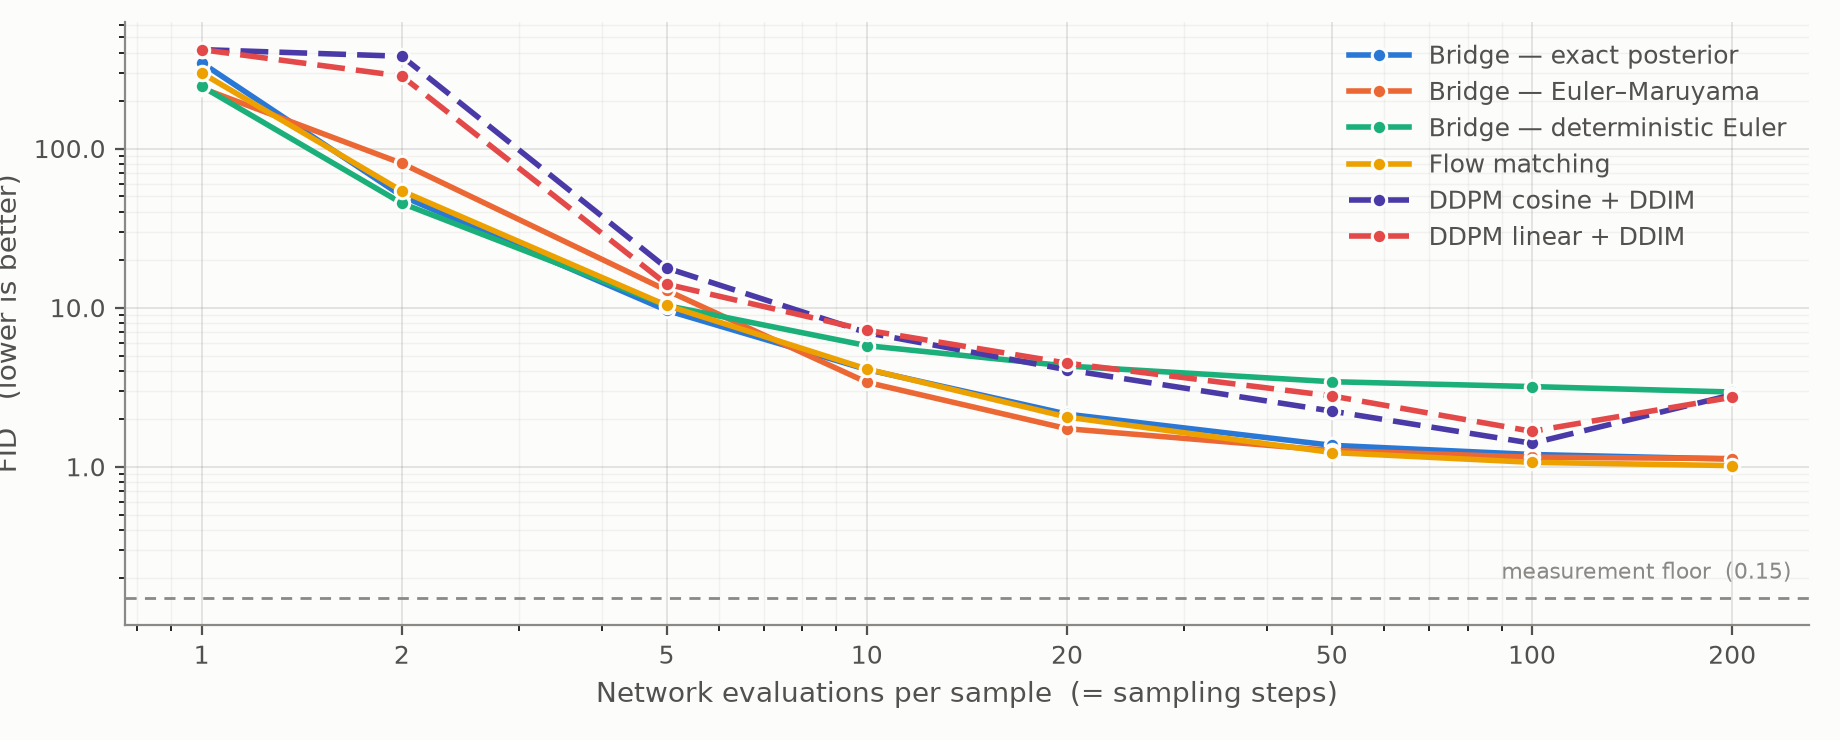
\includegraphics[width=0.97\textwidth]{../runs/figures/mnist_headline_compact.png}
\caption*{\scriptsize\textbf{Sampling efficiency on MNIST at matched budget.}
FID vs.\ network evaluations per sample; six schemes sharing one 7.28M UNet,
AdamW $2\!\times\!10^{-4}$, EMA $0.9999$, batch 128, 40{,}000 steps and identical
scoring code --- only the process and its sampler differ. 50{,}000 samples per
point against the full training split; the dashed rule at $0.15$ is the floor
measured between disjoint real subsets of the same size. Bridge leads at 10--20
evaluations, flow matching from 50. Deterministic Euler (green) is what the
original evaluated: it converges to ${\sim}3\times$ the floor excess of the
correct samplers. The DDPM curves turn upward after 100 evaluations; checked
against an alternative DDIM timestep grid, this is a real consequence of the
cosine schedule's near-zero terminal SNR, not an implementation artefact.}
\end{figure}

\end{document}
